% THIS TEMPLATE IS A WORK IN PROGRESS

\documentclass{article}
\usepackage[brazil]{babel}
\usepackage[utf8]{inputenc}
\usepackage{hyperref}
\usepackage{fancyhdr}
\usepackage{graphicx}
%\lhead{\includegraphics[width=0.2\textwidth]{nyush-logo.pdf}}
\fancypagestyle{firstpage}{%
  \lhead{Departamento de Engenharia Elétrica - UFMG}
  \rhead{
  %%%% COMMENT OUT / UNCOMMENT THE LINES BELOW TO FIT WITH YOUR MAJOR(S)
  Engenharia de Sistemas  }
}

%%%% PROJECT TITLE
\title{ Modelagem Inicial do Guindaste usando CoppeliaSim}

%%%% NAMES OF ALL THE STUDENTS INVOLVED (first-name last-name)
\author{João Victor de Castro Alves,\\
        Juliana Assis Alves\\
        Pierre Victor da Silva Sousa \\
        Roberto Pires Oliveira \\
        Vítor Corrêa Silva \\
        \\
        GRUPO D}

\date{\vspace{-5ex}} %NO DATE



\begin{document}
\maketitle
\thispagestyle{firstpage}
\section{Introdução}

    Nesse trabalho iremos modelar a versão básica do guindaste com leves modificações 
    no software CoppeliaSim. Isso tem como objetivo  não só comprovar o entendimento do grupo 
    sobre o software e a tarefa mas também consolidar os conhecimentos adquiridos tendo em vista 
    que o projeto modelado deverá ser implementado em sua forma física.
    
\section{Definição do Problema}

    O primeiro passo para desenvolver o modelo é estabelecer quais são as diretivas que iram 
    guiar nosso design. Tendo em vista que nenhuma restrição de dimensão ou design foi diretamente feita pelo 
    professor, iremos usar somente as carcteristicas do problema que o modelo deve solucionar.

    A definição formal do nosso problema pode ser escrita como :

    \begin{center}
        "O guindaste deve ser capaz de pegar uma moeda de 50 centavos a uma altura de 7mm e 150mm de 
        distância do guindaste levar essa moeda até uma base, também a 150mm de distância e com uma 
        altura de até 220mm."
    \end{center}

\section{Modelagem das peças}   

    Utilizando somente essas definições é possível já extrair algumas das medidas físicas que nosso 
    guindaste deve ter. Permitindo assim a criação de um modelo suficientemente satisfatório. Sendo 
    assim é possível escrever essas definições da seguinte forma :

    \begin{itemize}
        \item A altura da torre deve exceder \(220mm\).
        \item O comprimento da lança deve ser, no mínimo, \(150mm\).
        \item O atuador deve ser capaz de acoplar e manter acoplado por tempo indeterminado um objeto metálico de \(8g\).
    \end{itemize}
    \subsection{Base}

        A base é responsável por garantir a estabilidade de toda a estrutura do guindaste. Temos que garantir 
        que a base tenha tamanho e peso suficiente para garantir que o guindaste não caia, estando ele 
        carregado ou não. Portanto a peça que será usada terá as seguintes caractéristicas :
        \begin{itemize}
            \item Tipo : Cuboid
            \item Dimensões : \(70mm\) x \(70mm\) x \(20mm\)
            \item Massa : \(200g\)
        \end{itemize}
    \subsection{Torre}

        A Torre precisa atender a restrição de altura tendo uma nível razoável de "folga", e ainda sendo factível 
        que esta torre consiga carregar a Lança estando ou não em movimento. Portanto a peça que será usada terá 
        as seguintes caractéristicas :
        \begin{itemize}
            \item Tipo : Cuboid
            \item Dimensões : \(50mm\) x \(50mm\) x \(300mm\)
            \item Massa : \(450g\)
        \end{itemize}
    \subsection{Lança}

        A lança é responsável por mover atuador até a posição alvo e deve ser capaz de aguentar tanto o 
        peso da carga quanto da estrutura do atuador
        \begin{itemize}
            \item Tipo : Cuboid
            \item Dimensões : \(250mm\) x \(30mm\) x \(15mm\)
            \item Massa : \(200g\)
        \end{itemize}
    \subsection{Contrapeso}

        O contrapeso tem a função de evitar o desequilíbrio da Lança e garantir que o guindaste 
        não tombe mesmo com o peso da carga. 
        \begin{itemize}
            \item Tipo : Cuboid
            \item Dimensões : \(30mm\) x \(30mm\) x \(30mm\)
            \item Massa : \(120g\)
        \end{itemize}
    \subsection{Atuador}

        O atuador usado será feito de forma customizada no software de forma que sua geometria é de 
        escolha livre. A geometria escolhida será a de um pequeno cilindro, buscando mimetizar a peça 
        utilizada na versão física a ser construída. Portanto :
        \begin{itemize}
            \item Tipo : Cylinder
            \item Dimensões : \(30mm\) x \(30mm\) x \(60mm\)
            \item Massa : \(300g\)
        \end{itemize}
    \subsection{Base do Atuador}

        Como o atuador será movido tbm horizontamente ele precisará de uma base própria que terá as seguintes caracteristicas:
        \begin{itemize}
            \item Tipo : Cuboid
            \item Dimensões : \(30mm\) x \(30mm\) x \(30mm\)
            \item Massa : \(30g\)
        \end{itemize}
    \section{Sensoriamento}

        Para ser possível ter o set completo de funcionalidades visando controle estável do guindaste será adicionado
        sensoriamento especificamento um tipo de sensor:
        \subsection{Sensor de Distância}

            Será usado um sensor de distância, especificamente do tipo raio, para calcular a distância entre o atuador 
            e tudo que está logo abaixo. As caracteristicas de configuração podem ser vistas abaixo :
            \begin{itemize}
                \item Tipo : Ray
                \item OffSet = \(5mm\)
                \item Distância Máxima = \(250mm\)
            \end{itemize}
        
    \section{Juntas}

        Juntas são objetos que tem o a função de simular movimento de uma estrutura em relação a outra. Esse movimento foi
        pode ter múltiplos parâmetros definidos porém para a essa iteração da simulação usaremos somente dois. O módulo máximo 
        de velocidade e o torque máximo.
        \subsection{Suporte}

            A junta de suporte tem como objetivo garantir a união da torre a base gerando assim estabilidade para o guindaste. Sua velocidade estará definida como zero e seu torque
            terá um valor simbólico de 100 N, buscando dar rubustez ao modelo:
            \begin{itemize}
                \item \(\left|\vec{V_{max}}\right| = 0\)
                \item \(T_{max} = 200\)
            \end{itemize}
        \subsection{Plano XY}
            \begin{itemize}
                \item \(\left|\vec{V_{max}}\right| = 20^{\circ}/S\)
                \item \(T_{max} = 200\)
            \end{itemize}
        \subsection{Eixo Z}
            \begin{itemize}
                \item \(\left|\vec{V_{max}}\right| = 6\cdot 10^{-2} m/S\)
                \item \(T_{max} = 100\)
            \end{itemize}
        \subsection{Alinhamento Horizontal}

            Assim como no vídeo, o guindaste em questão também tera três graus de liberdade portanto é necessário uma junta 
            prismática para gerar esse movimento. Ela terá as mesmas limitações da junta do Eixo Z.
            \begin{itemize}
                \item \(\left|\vec{V_{max}}\right| = 6\cdot 10^{-2} m/S\)
                \item \(T_{max} = 100\)
            \end{itemize}
    \section{API}

        Todo o controle do modelo será feito via API usando a linguagem Python. Para isso as seguintes classes e métodos foram desenvolvidos. 
        \subsection{Template}

            Para ser possível iteragir com todas as estruturas de forma padrão usando o handle será criada a classe template object, que irá conter além do handle do objeto 
            a que se refere, o canal de comunicação para a simulção. Sendo esse um parâmetro compartilhado entre múltiplas instâncias. Todas as classe que foram definidas a 
            seguir tendo essa classe ou uma classe filha como parente.
        \subsection{Juntas}

            Para esse modelo a funcionalidade de Control Loop será usada na junta. É uma modalidade aonde a velocidade máxima da junta é definida, e só a sua posição é controlada 
            via API. Para isso foram definidos dois métodos :
            \begin{itemize}
                \item getPosition : Retorna a posição da junta em relação aos seus limites superior e inferior.
                \item setPosition : Define a posição objetivo para a junta em relação aos seu limite superior e inferior
            \end{itemize}
        \subsubsection{Junta de Revolução}

            A gente de revolução não apresenta nenhum método novo porém tem os métodos anteriores modificados para trabalharem com dados em radianos e em graus.
        \subsubsection{Junta Prismática}

            Não há nenhuma modificação em relação a classe mãe 'Juntas', a existência dessa classe é puramente para future-proofing e clareza de código. 
        \subsection{Sensor de Distância}

            A classe do sensor de distância é derivada da classe 'Objeto' e possui o método necessário para ler e interpretar as leituras do sensor de distância.
            \begin{itemize}
                \item detect : Retorna o handle, assim como a distânca do objeto detectado. Caso não encontre um objeto retorna o valor infinito.
            \end{itemize}
    \section{Atuador}

            O atuador é por sí só um modelo autoral que necessita uma seção própria. Seu modelo consiste em três peças:
            \begin{itemize}
                \item Corpo : Consiste em un cilíndro de dimensões já explicitadas em sessões anteriores e tem a função de representar o corpo do imã que será usado na vida real.
                \item Sensor de Força : Será usada simplesmente como um link entre o corpo e o objeto alvo, como nenhuma de suas funcionalidade está sendo utlizada não se mostrou necessário descrever seu funcionamento.
                \item Sensor de Distância : O mesmo tipo de sensor usado para medir a distância entre a ferramenta e o chão, entretanto esse apresenta um range de somente \(20mm\).
            \end{itemize}
            \subsection{Comportamento}
                
                A proposta para o modelo de imã implementado é que utilizando o sensor de distância para encontrar o objeto no alcance de magnetização, o mesmo seja linkado a árvore do sensor de força 
                estabelecendo a ligação entre ele e o corpo do modelo e permitindo movimenta-lo até o destino e deposita-lo lá.
                
                Para permitir essa modelagem foram usadas funções da API Regular que retorna afetam diretamente a árvore de hierárquia de cena. Essas funções permitem que possamos fazer a inserção e retirada do objeto desejado da ramo desejado da árvore,
                durante a execução da simulação. Não hávera muitos detalhes do código implementado pois não se mostra necessário para esse relatório.
            
    \section{Resultados}
            
            Nesta sessão seram exibidos os resultados da modelagem, primeiramente, a árvore de hierarquia de cena final do modelo :
                \begin{figure}[h]
                    \centering
                    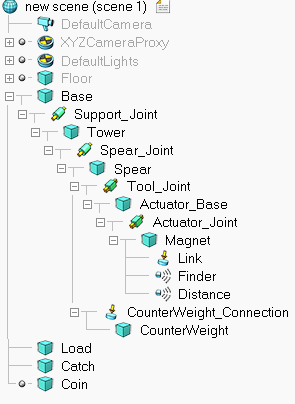
\includegraphics[scale = .4]{images/Tree.png}
                \end{figure}
            
            % \pagebreak

            O resultado final do modelo pode ser visto na imagem a seguir : 

                \begin{figure}[h]
                    \centering
                    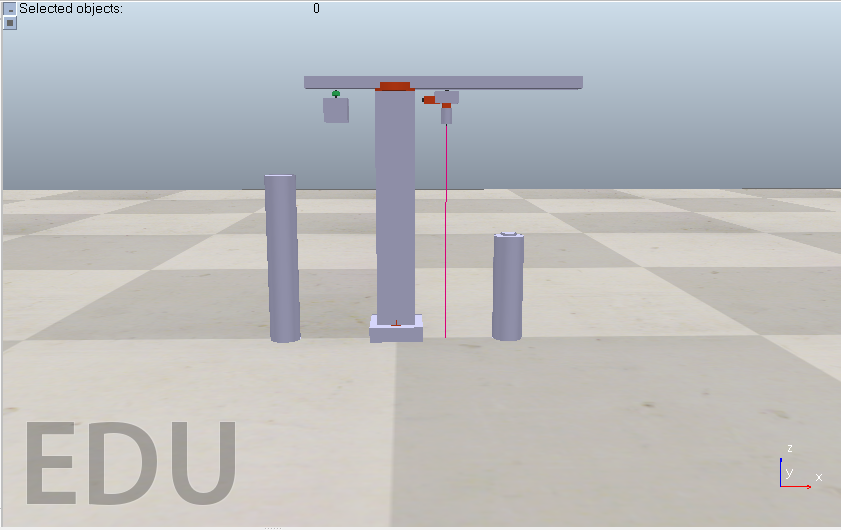
\includegraphics[scale = .4]{images/Model.png}
                \end{figure}

            Para ser possível controlar esse modelo de forma intuitiva e prática uma GUI básica foi programada usando o TKinter, uma biblioteca de desenvolvimento de 
            interfaces em python.

                \begin{figure}[h]
                    \centering
                    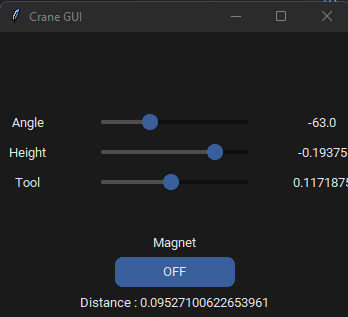
\includegraphics[scale = .4]{images/GUI.png}
                \end{figure}

            Para ser possível ver o modelo em pleno funcionamento é necessário acesssar o seguinte link \url{https://youtu.be/rzIPiQRTQPA}
\bibliographystyle{IEEEtran}
\bibliography{references}
\begin{itemize}
    \item COPPELIA REGULAR API, Dísponivel em : \url{https://www.coppeliarobotics.com/helpFiles/en/apiFunctions.htm}. Acessado em 2 de Maio de 2022
    \item V-REP Beginners Tutorial, Dísponivel em \url{https://www.youtube.com/playlist?list=PLxtIrkqXXpsg2OiTdisdZ59rj_47a886x}. Acessado em 2 de Maio de 2022
\end{itemize}

\end{document}
